\chapter{Session Management Testing}

	At the core of any web-based application is the way in which it maintains state and thereby 
	controls user-interaction with the site. Session Management broadly covers all controls on 
	a user from  authentication to leaving the application. HTTP is a stateless protocol, meaning 
	that web servers respond to client requests without linking them to each other. Even simple
	application logic requires a user's multiple requests to be associated with each other across 
	a "session”. Most popular web application environments, such as ASP and PHP, provide developers 
	with built-in session handling routines. Some kind of identification token will typically be issued, 
	which will be referred to as a “Session ID” or Cookie.

	\begin{figure}[H]
		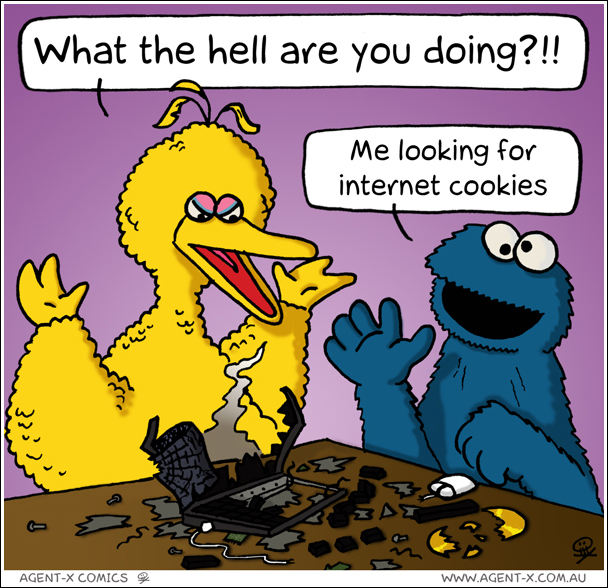
\includegraphics[scale=0.4]{pics/cookie.jpg}
	\end{figure}

	\clearpage
	\section{Session Management Schema}

		This describes how to analyse a Session Management Schema, with the goal to understand how 
		the Session Management mechanism has been developed and if it is possible to break it to 
		bypass the user session. It explains how to test the security of session tokens issued to 
		the client's browser: how to reverse engineer a cookie, and how to manipulate cookies
		to hijack a session.

		In order to avoid continuous authentication for each page of a website or service, web applications implement various mechanisms to store and validate credentials for a pre-determined timespan.
		These mechanisms are known as Session Management and, while they're most important in order to increase the ease of use and user-friendliness of the application.

		Cookies are used to implement {\bf session management}. In a nutshell, when a user accesses an 
		application which needs to keep track of the actions and identity of that user across multiple
		requests, a cookie (or more than one) is generated by the server and sent to the client. 
		The client will then send the cookie back to the server in all following connections until 
		the cookie expires or is destroyed. The data stored in the cookie can provide to the server
		a large spectrum of information about who the user is, what actions he has performed so far, 
		what his preferences are, etc. therefore providing a state to a {stateless protocol like HTTP}.
		
		A typical example is provided by an {\bf online shopping cart}. Throughout the session of a user, 
		the application must keep track of his identity, his profile, the products that he has chosen to 
		buy, the quantity, the individual prices, the discounts, etc.
		Cookies are an efficient way to store and pass this information back and forth (other methods are 
		URL parameters and hidden fields).
		
		Due to the importance of the data that they store, cookies are therefore vital in the overall 
		security of the application. Being able to tamper with cookies may result in hijacking the 
		sessions of legitimate users, gaining higher privileges in an active session, and in general
		influencing the operations of the application in an unauthorized way. 

		Usually the main steps of the attack pattern are the following:
			\begin{itemize}
				\item {\bf Cookie collection:} collection of a sufficient number of cookie samples;
				\item {\bf Cookie reverse engineering:} analysis of the cookie generation algorithm;
				\item {\bf Cookie manipulation:} forging of a valid cookie in order to perform the 
				attack. This last step might require a large number of attempts, depending on how the 
				cookie is created (cookie brute-force attack).
				\item {\bf Cookie overflow:} Strictly speaking, this attack has a different nature. Instead 
				of getting a valid cookie, our goal is to overflow a memory area, thereby interfering
				with the correct behavior of the application and possibly injecting (and remotely 
				executing) malicious code.
			\end{itemize}

		\subsection{Cookie Collection and Session Analysis}

			The first step required in order to manipulate the cookie is obviously to understand how 
			the application creates and manages cookies. For this task, we have to try to answer the
			following questions: 

			{\bf How many cookies are used by the application?} \\
			Surf the application. Note when cookies are created. Make a list of received cookies, 
			the page that sets them (with the set-cookie directive), the domain for which they are 
			valid, their value, and their characteristics.

			{\bf Which parts of the application generate and/or modify the cookie?} \\
			Surfing the application, find which cookies remain constant and which get modified. 
			What events modify the cookie?

			{\bf Which parts of the application require this cookie in order to be accessed and utilized?} \\
			Find out which parts of the application need a cookie. Access a page, then try again without 
			the cookie, or with a modified value of it. Try to map which cookies are used where.
			A spreadsheet mapping each cookie to the corresponding application parts and the related 
			information can be a valuable output of this phase.

			The session tokens (Cookie, SessionID or Hidden Field) themselves should be examined to 
			ensure their quality from a security perspective. They should be tested against criteria 
			such as their randomness, uniqueness, resistance to statistical and cryptographic analysis 
			and information leakage.


		\subsection{Token structure and Information Leakage}
			The first stage is to examine the structure and content of a Session ID provided by 
			the application. A common mistake is to {\bf include specific data} in the Token instead 
			of issuing a generic value and referencing real data at the server side. 
			If the Session ID is {\bf clear-text}, the structure and pertinent data may be immediately
			obvious as the following: \\
			{\bf Clear-text:} {\color{blue} 192.168.100.1:owaspuser:password:15:58} \\
			{\bf Hybrid:} {\color{blue} owaspuser:192.168.100.1: a7656fafe94dae72b1e1487670148412}

			If part or the entire token appears to be encoded or hashed, it should be compared to 
			various techniques to check for obvious obfuscation. Having identified the type of 
			obfuscation, it may be possible to decode back to the original data.

				\begin{figure}[H]
					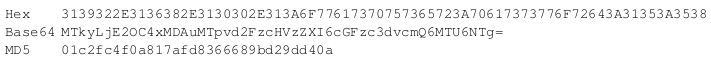
\includegraphics[width=\textwidth]{pics/cookies.png}
				\end{figure}

			A simple analysis of the tokens should immediately reveal any obvious patterns. 
			For example, a 32 bit token may include 16 bits of static data and 16 bits
			of variable data. This may indicate that the first 16 bits represent a fixed attribute 
			of the user – e.g. the username or IP address. If the second 16 bit chunk is incrementing 
			at a regular rate, it may indicate a sequential or even time-based element to the token
			generation.The following areas should be addressed during the single and multiple Session 
			ID structure testing:

				\begin{itemize}
					\item What parts of the Session ID are static?
					\item What clear-text confidential information is stored in the Session ID? 
					E.g. usernames/UID, IP addresses
					\item What easily decoded confidential information is stored?
					\item What information can be deduced from the structure of the Session ID?
					\item What portions of the Session ID are static for the same login conditions?
					\item What obvious patterns are present in the Session ID as a whole, or individual
					portions?
				\end{itemize}

		\subsection{Session ID Predictability and Randomness}
			Analysis of the variable areas (if any) of the Session ID should be undertaken to 
			establish the existence of any recognizable or predictable patterns. 
			In analyzing Session ID sequences, patterns or cycles, static elements and client 
			dependencies should all be considered as possible contributing elements to the structure 
			and function of the application:
				\begin{itemize}
					\item Are the Session IDs provably random in nature?
					\item Do the same input conditions produce the same ID on a subsequent run?
					\item Are the Session IDs provably resistant to statistical or cryptanalysis?
					\item What elements of the Session IDs are time-linked?
					\item What portions of the Session IDs are predictable?
					\item Can the next ID be deduced, given full knowledge of the generation algorithm 
					and previous IDs
				\end{itemize}

		\subsection{Cookie Reverse Engineering}
			Now that we have enumerated the cookies and have a general idea of their use, it is time to 
			have a deeper look at cookies that seem interesting. Which cookies are we interested in? 
			A cookie, in order to provide a secure method of session management, must combine several
			characteristics, each of which is aimed at protecting the cookie from a different class 
			of attacks. These characteristics are summarized below:

				\begin{enumerate}
					\item {\bf Unpredictability:} a cookie must contain some amount of hard-to-guess 
					data. The harder it is to forge a valid cookie, the harder is to break into 
					legitimate user's session. If an attacker can guess the cookie used in an active 
					session of a legitimate user, he/she will be able to fully impersonate that user 
					(session hijacking). In order to make a cookie unpredictable, random values 
					and/or cryptography can be used.
					\item {\bf Tamper resistance:} a cookie must resist malicious attempts of 
					modification. If we receive a cookie like IsAdmin=No,  it is trivial to modify it 
					to get administrative rights, unless the application performs a double check 
					(for instance, appending to the cookie an encrypted hash of its value)
					\item {\bf Expiration:} a critical cookie must be valid only for an appropriate 
					period of time and must be deleted from disk/memory afterwards, in order to avoid 
					the risk of being replayed. This does not apply to cookies that store non-critical 
					data that needs to be remembered across sessions (e.g., site look-and-feel)
					\item {\bf “Secure” flag:} a cookie whose value is critical for the integrity of 
					the session should have this flag enabled in order to allow its transmission only 
					in an encrypted channel to deter eavesdropping.
				\end{enumerate}

				\begin{figure}[H]
					\centering
					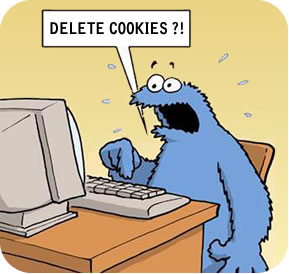
\includegraphics[scale=0.5]{pics/deleteCookies.jpg}
				\end{figure}

			The approach here is to {\bf collect a sufficient number of instances of a cookie} and 
			start looking for {\bf patterns} in their value. The exact meaning of “sufficient” can vary 
			from a handful of samples, if the cookie generation method is very easy to break, to
			several thousands, if we need to proceed with some mathematical analysis.

			It is important to pay particular attention to the {\bf workflow of the application}, 
			as the state of a session can have a heavy impact on collected cookies: a cookie 
			collected before being authenticated can be very different from a cookie obtained
			after the authentication.

			Another aspect to keep into consideration is {\bf time}: always record the exact time 
			when a cookie has been obtained, when there is the possibility that time plays a role 
			in the value of the cookie (the server could use a timestamp as part of the
			cookie value).

			{\bf Analyzing the collected values}, try to figure out all variables that could have 
			influenced  the cookie value and try to vary them one at the time. Passing to the server 
			modified versions of the same cookie can be very helpful in understanding how the 
			application reads and processes the cookie.

		\subsection{Brute Force Attacks}
			Brute force attacks inevitably lead on from questions relating to predictability and 
			randomness. The variance within the Session IDs must be considered together with 
			application session durations and timeouts. If the variation within the Session
			IDs is relatively small, and Session ID validity is long, the likelihood of a successful 
			brute-force attack is much higher. A long Session ID (or rather one with a great deal 
			of variance) and a shorter validity period would make it far harder to succeed in a
			brute force attack.

		\clearpage
		\subsection{Cookie Manipulation}
			Once you have squeezed out as much information as possible from the cookie, it is 
			time to start to modify it. The methodologies here heavily depend on the results 
			of the analysis phase, but we can provide some examples:

			{\bf Example 1: Guessable Cookie} \\
			An example of a cookie whose value is easy to guess and that can be used to impersonate 
			other users can be found in OWASP WebGoat, in the “Weak Authentication cookie” lesson. 
			In this example, you start with the knowledge of two username/password couples 
			(corresponding to the users 'webgoat' and 'aspect'). The goal is to reverse engineer 
			the cookie creation logic and break into the account of user 'alice'. 
			Authenticating to the application using these known couples, you can collect the 
			corresponding authentication cookies.

			\begin{figure}[H]
				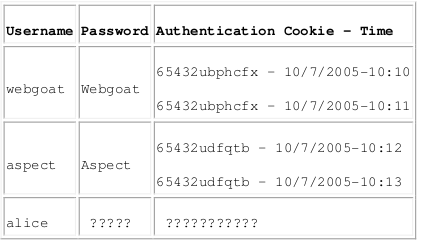
\includegraphics[scale=0.5]{pics/exampleCookie.png}
			\end{figure}

			First of all, we can note that the authentication cookie remains constant for the same 
			user across different logons, showing a first critical vulnerability to replay attacks: 
			if we are able to steal a valid cookie (using for example a XSS vulnerability), we
			can use it to hijack the session of the corresponding user without knowing his/her 
			credentials. Additionally, we note that the “webgoat” and “aspect” cookies have a 
			common part: “65432u”. So let's see the letter following each letter in “webgoat”:

			\begin{figure}[H]
				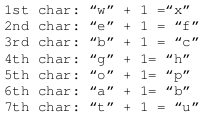
\includegraphics[scale=0.5]{pics/webgoat.png}
			\end{figure}

			We obtain “xfchpbu”, which inverted gives us exactly “ubphcfx”. The algorithm fits 
			perfectly also for the user 'aspect', so we only have to apply it to user 'alice'.
			Bingo! Now can the application identifies us as “alice” instead of “webgoat”.

		\subsection{Brute Force}

		The use of a brute force attack to find the right authentication cookie, could be a 
		heavy time consuming technique. Foundstone Cookie Digger can help to collect a large 
		number of cookies, giving the average length and the character set of the cookie. 
		In advance, the tool compares the different values of the cookie to check how many 
		characters are changing for every subsequent login. If the cookie values do not 
		remain the same on subsequent logins, Cookie Digger gives the attacker longer periods 
		of time to perform brute force attempts. In the following table we show an example 
		in which we have collected all the cookies from a public site, trying 10 authentication 
		attempts. For every type of cookie collected you have an estimate of all the possible 
		attempts needed to “brute force” the cookie.

		\begin{figure}[H]
			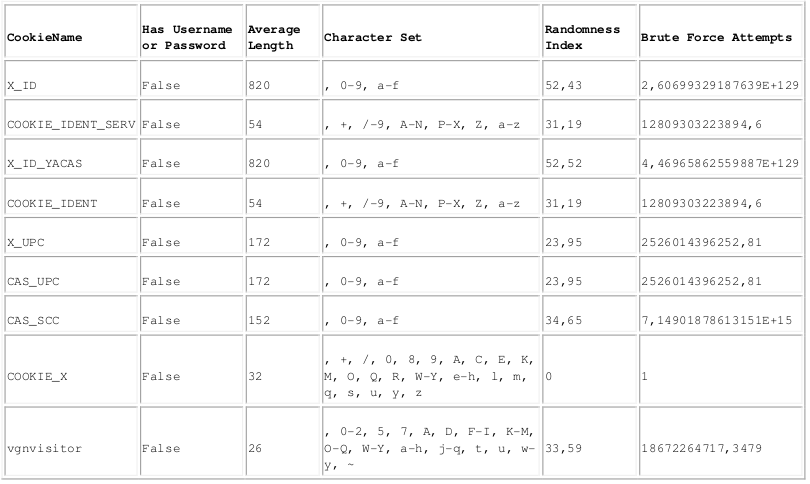
\includegraphics[width=\textwidth]{pics/bruteforce.png}
		\end{figure}

		\subsection{Overflow}
			Since the cookie value, when received by the server, will be stored in one or more 
			variables, there is always the chance of performing a boundary violation of that 
			variable. Overflowing a cookie can lead to all the outcomes of buffer overflow
			attacks. A Denial of Service is usually the easiest goal, but the execution of 
			remote code can also be possible. Usually, however, this requires some detailed 
			knowledge about the architecture of the remote system, as any buffer overflow
			technique is heavily dependent on the underlying operating system and memory 
			management in order to correctly calculate offsets to properly craft and align 
			inserted code.

	\section{Cookies Attributes}

		Cookies are often a key attack vector for malicious users (typically targeting other users) 
		and, as such, the application should always take due diligence to protect cookies. In this 
		section, we will look at how an application can take the necessary precautions when assigning 
		cookies and how to test that these attributes have been correctly configured.

		As you can imagine, there are many different types of applications that need to keep track 
		of session state across multiple requests. The primary one that comes to mind would be an 
		online store. As a user adds multiple items to a shopping cart, this data needs to be retained 
		in subsequent requests to the application. Cookies are very commonly used for this task and 
		are set by the application using the Set-Cookie directive in the application's HTTP response, 
		and is usually in a name=value format. Once an application has told the browser to use a 
		particular cookie, the browser will send this cookie in each subsequent request. 
		A cookie can contain data such as items from an online shopping cart, the price of these items, 
		the quantity of these items, personal information, user IDs, etc. D
		ue to the sensitive nature of information in cookies, they are typically encoded or encrypted 
		in an attempt to protect the information they contain. 

		Let's take a look at what attributes can be set for a cookie. 
		The following is a list of the attributes that can be set for each cookie and 
		what they mean:

		\begin{itemize}
			\item {\bf Secure} - This attribute tells the browser to only send the cookie if the 
			request is being sent over a secure channel such as HTTPS. If the application can be 
			accessed over both HTTP and HTTPS, then there is the potential that the cookie can be 
			sent in clear text.
			\item {\bf HttpOnly} - This attribute is used to help prevent attacks such as cross-site
			scripting, since it does not allow the cookie to be accessed via a client side script 
			such as JavaScript. 
			\item {\bf Domain} - This attribute is used to compare against the domain of the server 
			in which the URL is being requested. 
			\item {\bf Path} - In addition to the domain, the URL path can be specified for which 
			the cookie is valid. If the domain and path match, then the cookie will be sent in the 
			request.
			\item {\bf Expires} - This attribute is used to set persistent cookies, since the cookie 
			does not expire until the set date is exceeded. This persistent cookie will be used by 
			this browser session and subsequent sessions until the cookie expires. Once the expiration 
			date has exceeded, the browser will delete the cookie.
		\end{itemize}

	\section{Session Fixation}

	\section{Exposed Session Variables}

	\section{CSRF}

		CSRF is an attack which forces an end user to execute unwanted actions on a web application 
		in which he/she is currently authenticated. With a little help of {\bf social engineering} 
		(like sending a link via email/chat), an attacker may force the users of a web application 
		to execute actions of the attacker's choosing. A successful CSRF exploit can compromise end 
		user data and operation, when it targets a normal user. 